\chapter{Design}\label{ch:design}
%Is the central chapter of the work. Here the goal as well as the own ideas, evaluations, design decisions are presented. It can be worthwhile to play through different possibilities and then explicitly justify why one has chosen a particular one. This chapter should - at least in keywords - already be sketched out and written in keywords when a design is first defined. However, in a normal course of work, something will constantly change. The chapter must not become too detailed, otherwise the reader will be bored. It is very important to find the right level of abstraction. When writing, one should pay attention to the reusability of the text. (8-20 pages)

% 1. Decision: why AIE instead of DSP (mention config_block_design here) x
% 2. Decision: why Cooley-Tukey instead of reversed index technique (latter one used on one single kernel) x
% 3. Decision: what specific Cooley-Tukey decomposition x?
% 4. D: Using pkt streaming for data partition
% 5. D: Using PL for reordering between stages
% 6. D: Pipeling of the stages (maybe later)
% 7. D: Stream pkts into buffers (stalling problem) / why no ping pong buffers
% 8. D: precalculated twiddle factors
% 9. D: how si the vector unit used

This chapter provides a detailed explanation of the design of the \ac{fft} implementation, with a focus on both hardware and software decisions. Beforehand an the system requirements described in section \ref{sec:req}, which are driven by the need to support large Fourier Transforms for synthetic aperture as described in section \ref{sec:fbi}, will be translated into constraints for the design. The overall goal will be to calculate 256 different \ac{fft}s with a size of $2^{18}$ each within 30 ms.

\section{Constraints}
As outlined in the initial design goals, the algorithm developed in this thesis aims to enable real-time processing capabilities for a system with 256 receivers and 10 senders, requiring a high level of performance for \ac{fft} computation. For each frame of the desired 30 frames per second stream, each of the 256 receivers must process an \ac{fft} based on  $2^{18}$ data points sampled from a 4 ms signal at 65.536 MHz with a 16-bit resolution per data point. This translates to a total of 256 \ac{fft}s needing completion within the 30 ms window.\par
In light of these goals, several constraints emerge, notably in terms of memory and processing speed. Each $2^{18}$-point \ac{fft} utilizes 64-bit (8 bytes) precision per complex data point, given the \ac{adc}'s fixed bit resolution and property of the complex number to have a real and an imaginary part. This leads to a memory demand of approximately 2.1 MB per \ac{fft}. As discussed in Section \ref{sec:versal}, the Versal platform's AI Engines provide a combined memory capacity of 12.8 MB, theoretically allowing for four concurrent \ac{fft} computations. However, to manage memory allocation effectively across AI engine tiles and account for data streaming and precomputed values, the design optimizes resource allocation by processing one \ac{fft} at a time. To compensate for this all the \ac{fft}s need to be calculated sequentially within the 30 ms limit. The further analysis of this issue will show that this becomes possible as now more calculation units are now available for this particular calculation step.\par
With this design decision, timing constraints intensify. To maintain the 30 ms target, each \ac{fft} must complete within 0.117 ms. Operating at 1.25 GHz, the AI Engines provide a processing window of 146,250,000 instructions per \ac{fft}. These constraints shape the algorithm optimization, guiding the memory and processing flow throughout the system. The following sections detail the architectural choices implemented to meet these stringent requirements, focusing on efficient memory management and the distribution of computational resources across the AI Engine array.

\begin{figure}[h]
    \centering
    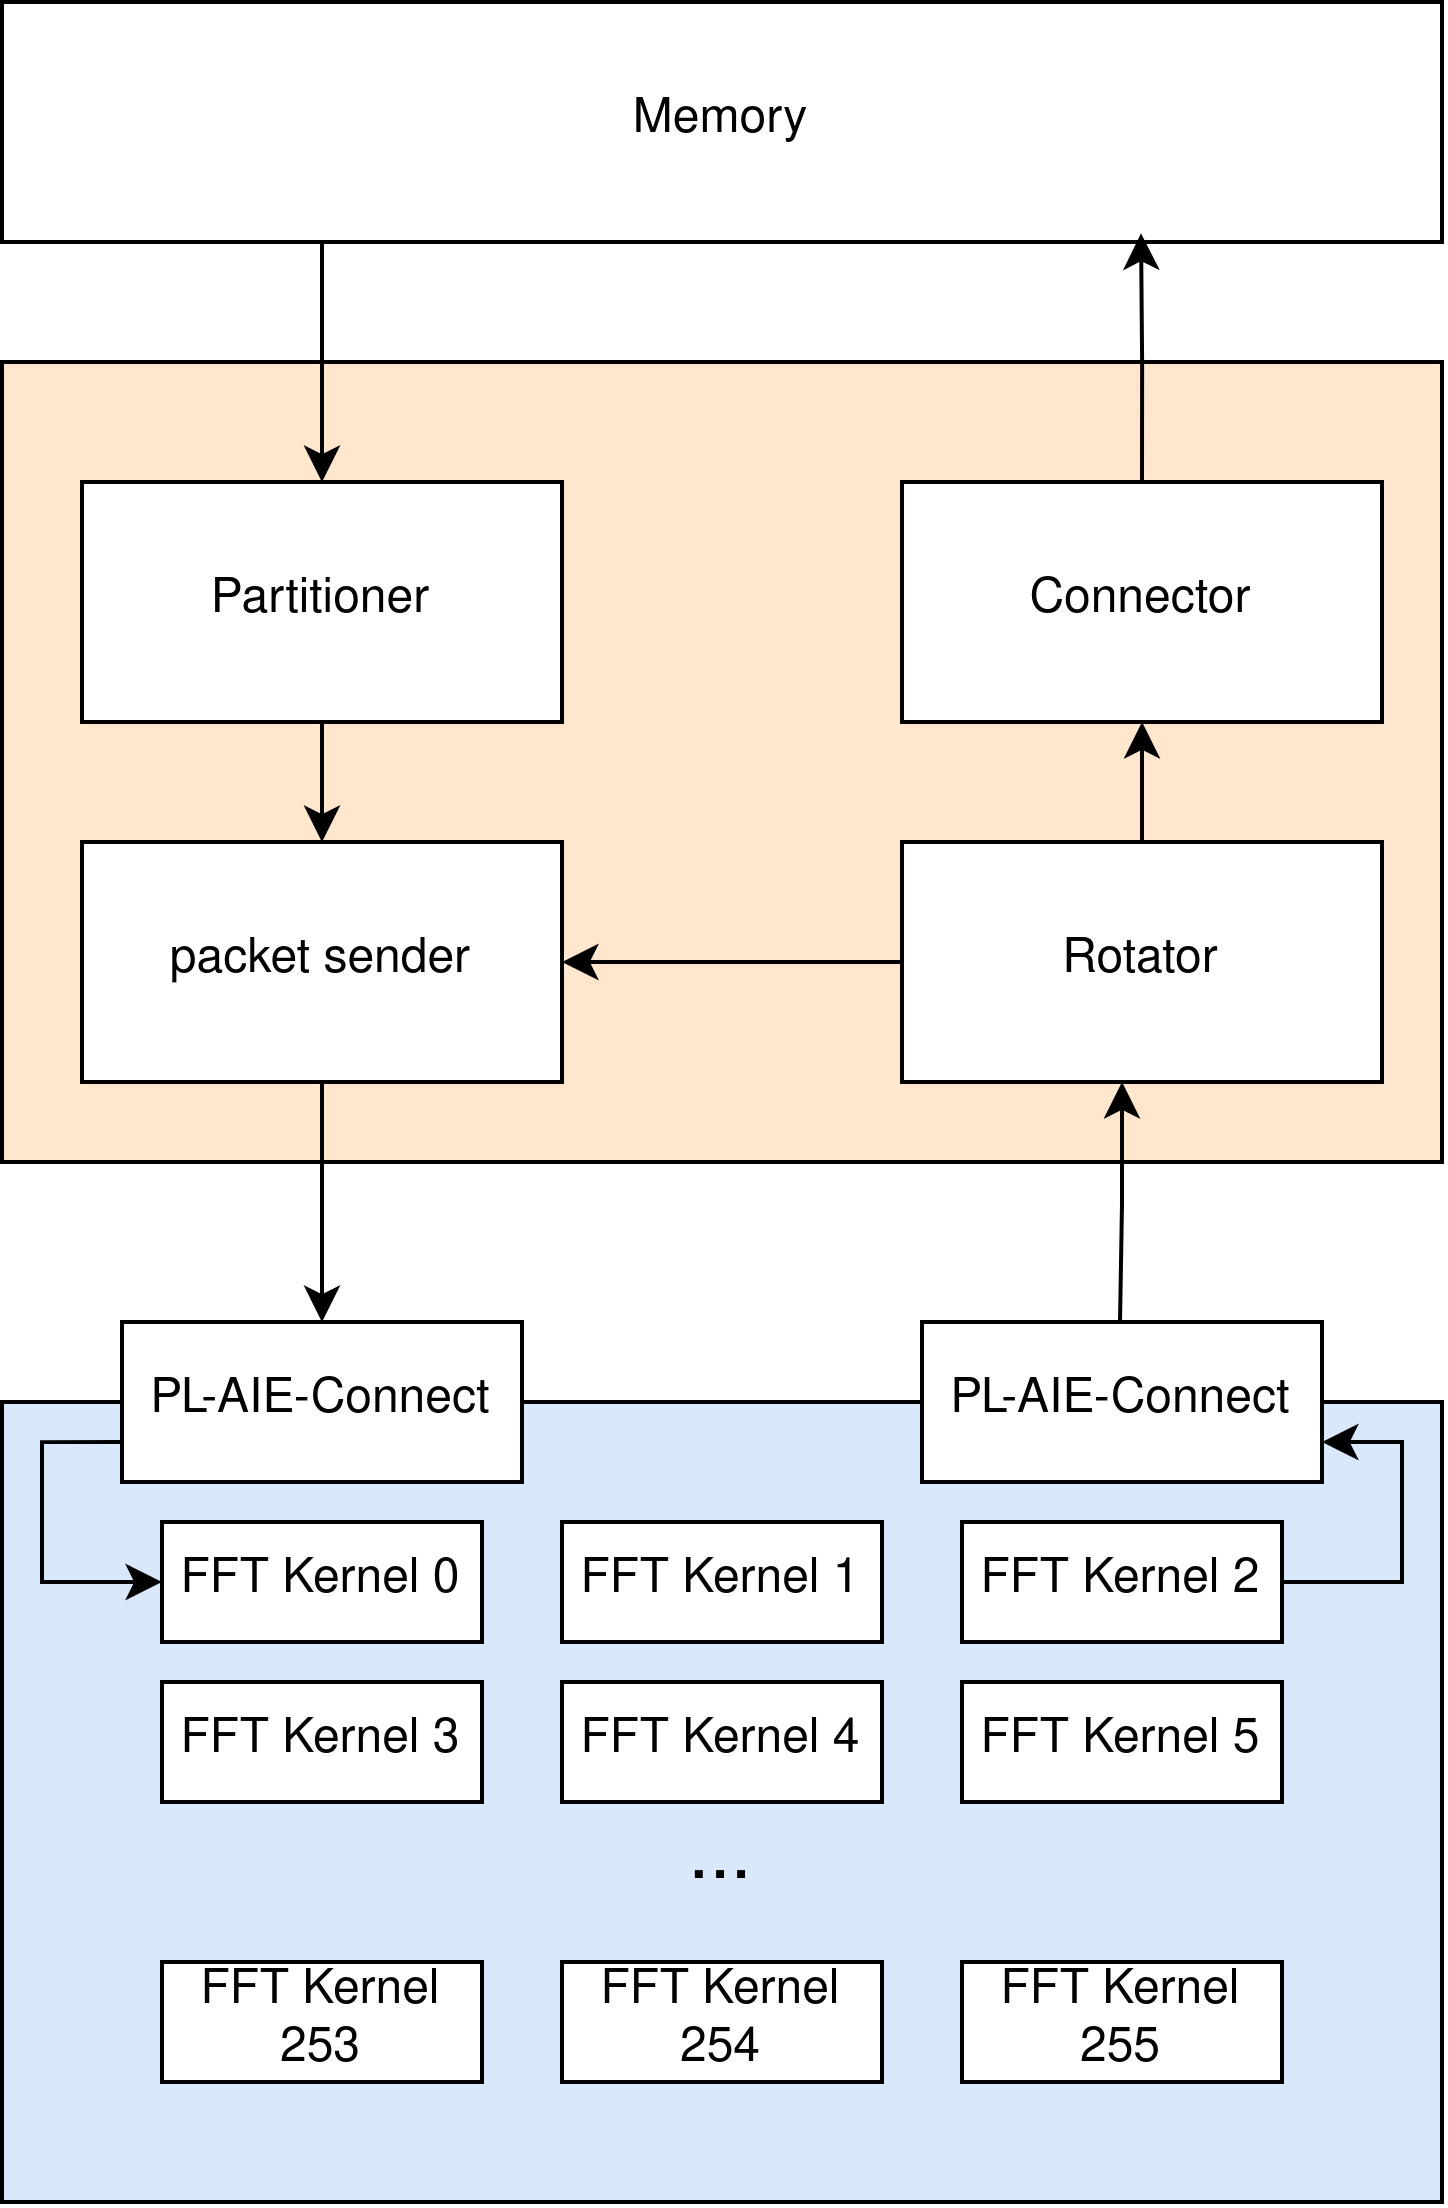
\includegraphics[width=0.5\textwidth]{images/overview.png}
    \captionsetup{justification=centering}
    \caption{Overview over the major building blocks in \ac{pl} and AI Engines}
        The general structure of the algorithm divided into its main building blocks. The yellow box shows the parts located in the \ac{pl} while the blue box outlines the kernels within the AI Engines.
    \label{fig:overview}
\end{figure}

\section{Overall Structure}
A straightforward approach to reduce the number of sequential instructions is to parallelize the algorithm. While this does not necessarily decrease the total number of instructions, it does reduce the number of instructions that need to be executed sequentially within the specified time frame. This is because two instructions computed in parallel contribute only once to the time constraint. An effective way to parallelize an \ac{fft} is by utilizing the Cooley-Tukey algorithm described in section \ref{sec:ft}. For practical reasons, I chose to decompose the $2^{18}$-point \ac{fft} into smaller 1,024-point and 256-point \ac{fft}s. This structure allows to fully utilize the memory of one AI Engine tile which features four 8kb memory ranks. The buffer for the 1024-point \ac{fft} would be exactly 8kb large. This allows to fit the input and output buffer of one kernel exactly on to one memory bank each. Further this allows to reuse a the same memory structure for the 256-point \ac{fft}s as they are a divisor of 1024.In the following sections, I will describe the overall algorithm design, detailing how this decomposition is employed to optimize performance while meeting the design constraints.\par
The architecture of the system is divided into two key components: the \ac{pl} and the AI engines. Each of these components is further subdivided into smaller functional units. The central idea behind this design is the dataflow between these two components. Initially, data is streamed from the DDR memory through the \ac{pl} to the AI engines, where the first stage of the \ac{fft} computation is performed. Once this initial computation is completed, the data is transferred back to the \ac{pl}, where it is reordered in preparation for the second stage of processing. Subsequently, the data is streamed again into the AI engines, where the second stage of the \ac{fft} computation takes place. Finally, the processed data is written back to memory through the \ac{pl}. This dataflow structure is designed to optimize the utilization of both the \ac{pl} and the AI engines, ensuring efficient processing while adhering to the timing constraints discussed in previous sections.\par
As previously discussed, the \ac{pl} is responsible for managing the interaction with the RAM and controlling the data stream for the AI engines. The \ac{pl} consists of four main components, as illustrated in figure \ref{fig:overview}.The first component, the Partitioner, is primarily responsible for interacting directly with the DDR memory, handling the loading and reordering of input data. This ensures that the data is properly prepared for the subsequent stages of computation.The Packet Sender is the second component and can receive data streams from two sources: either from the Partitioner or from the Rotator. It packages these data streams into packets, which are then streamed to the AI engines for \ac{fft} computation.The Rotator, another key component, takes the data stream returned from the AI engines after the first \ac{fft} stage. It can either pass the data directly to the Connector or reorder it before sending it back to the Packet Sender for further \ac{fft} processing.\par
Finally, the Connector is responsible for writing the final \ac{fft} results back to the DDR memory. It abstracts the logical processing from memory access, ensuring a clear separation between the computational processes and the data storage operations.Together, these components coordinate the flow of data between memory, the \ac{pl}, and the AI engines, facilitating efficient handling of the large data volumes required for the \ac{fft} computations.\par
The second major building block, the AI engines, are organized differently than the \ac{pl}. They are connected to the \ac{pl} via specialized connection tiles (see section \ref{sec:versal}). As illustrated in the schematic, these connection tiles specifically link to the Packet Sender and Rotator. Each of these two building blocks is connected with 8 streams to these tiles. The connection tiles take the eight data streams they receive and split them into 32 packets each, which are then streamed to individual AI engine tiles. This configuration utilizes a total of 256 AI engine tiles. Each of these tiles implements the same kernel, which is capable of executing either a 1024-point \ac{fft} followed by a phase rotation or four separate 256-point \ac{fft}s. The appropriate mode is selected using a control word embedded in the data stream. After the computations are completed, the data is streamed back to the connection tiles, where the individual streams are repackaged into eight data streams before being sent back to the \ac{pl}. This structured approach to the AI engines enhances parallel processing capabilities, allowing for efficient execution of \ac{fft} calculations while maintaining a streamlined connection to the \ac{pl}.

\begin{figure}[h]
    \centering
    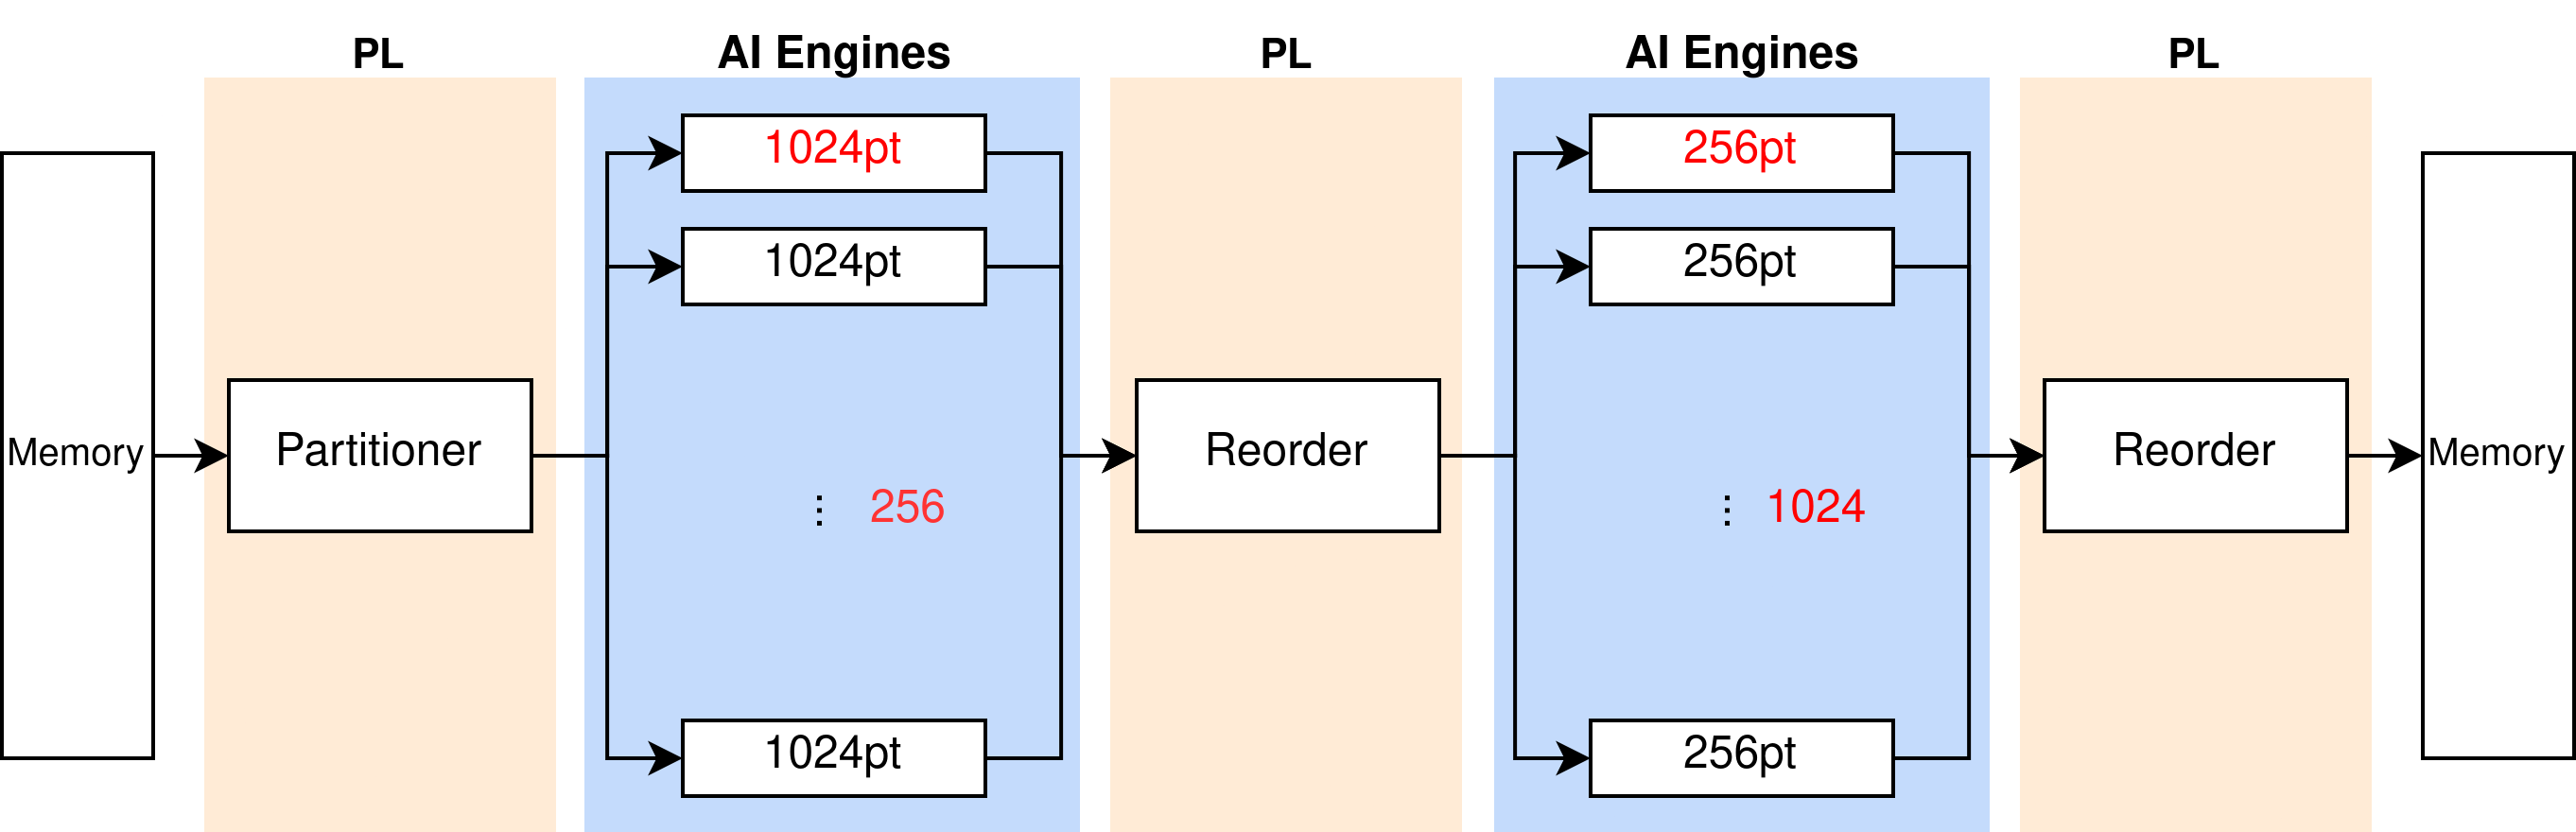
\includegraphics[width=1.0\textwidth]{images/prototype.png}
    \captionsetup{justification=centering}
    \caption{Pipelined algorithm design}
            Every vertical slice is independent from the other parts of the system. Yellow slices are implemented on the PL while blue slice are implemented as kernels on the AI Engines.
    \label{fig:pipelined}
\end{figure}

\section{Sequential or pipelined design}
As illustrated by the color coding in figure \ref{fig:overview}, the \ac{pl} (yellow )and the AI engines (blue) represent two distinct components that utilize different hardware. This distinction raises an important question regarding the potential for pipelining between these two stages. Implementing a pipelined approach could alleviate some of the design constraints discussed earlier, as the runtime constraint would no longer apply to the entire design, but only to the slowest pipeline stage. Figure \ref{fig:pipelined} presents a design that incorporates a pipelined approach. However, this design is not without its drawbacks and challenges, which will be explored in detail in this section.\par
The design depicted in the schematic closely resembles the previously described architecture. It features building blocks within the \ac{pl} that are responsible for partitioning and reordering data, alongside building blocks within the AI engines that perform the actual computations. The primary distinction in this design is that each building block operates as its own instance. This means that every implementation of a building block in the \ac{pl} occupies dedicated hardware resources, enabling it to run in parallel with other instances of the same block. In the schematic, this parallelism is represented by the slices, each symbolizing an independent implementation, in contrast to the shared implementations shown in figure \ref{fig:overview}. This concept similarly applies to the AI engines, where each kernel is implemented on its own tile. This architectural design facilitates a pipelined approach, allowing each of the vertical stages in figure \ref{fig:pipelined} to operate concurrently with the other stages. Such parallel execution enhances the overall throughput of the system and improves efficiency in handling the computational load.\par
One significant limitation of this design is resource allocation, especially considering the increased resource demands of the AI engines. While the \ac{pl} provides ample resources to implement multiple instances of identical building blocks, the AI engines face constraints due to the limited number of available tiles and the restricted memory capacity per tile. As outlined in section \ref{sec:versal}, each tile has a maximum memory of 32 KB. Not all of this memory can be allocated for storing data on which the \ac{fft} will be executed. As described in more detail in section \ref{sec:imp}, each AI engine requires two buffers—one for incoming unprocessed data and one for processed data. Consequently, each buffer is limited to only 8 KB of memory, with the remaining memory allocated for other internal data structures required by the algorithm. This constraint allows only the decomposition of the \ac{fft} into a maximum of 1024 and 256 \ac{fft}s. The assignment of AI engines follows accordingly: in the first stage, 256 tiles are allocated for the 1024 \ac{fft}s, while the second stage would ideally require 1024 tiles for the 256 \ac{fft}s. With only 400 tiles available, this configuration is infeasible. Even if four 256 \ac{fft}s were placed on each tile to fully utilize the 8 KB of memory in each second-stage kernel, 256 AI engines would still be needed for the second stage. This would result in a total of 512 AI engines, exceeding the 400-tile limit. Due to these limitations, it is not possible to pipeline the design for such a large \ac{fft} \cite{AMD_a_aie}.

\section{Programmable Logic kernels}
A critical question arising from the proposed design is the rationale behind incorporating \ac{pl} at all. At first glance, it may seem more practical to confine the design within the AI engines to avoid complications associated with differing clock domains and the need for multiple streaming interfaces between various hardware components. However, the use of \ac{pl} remains essential due to the specific structure of the data that needs to be processed. As described in section \ref{sec:ft}, the data must be reordered between the two stages of the \ac{fft} in such a way that the index value of the output from the first stage directly corresponds to the \ac{fft} that will process this output in the second stage. Specifically, the first output of the first \ac{fft} from the first stage serves as the first input for the first \ac{fft} of the second stage. Similarly, the second output of the first \ac{fft} from the first stage becomes the first input for the second \ac{fft} of the second stage, while the first output of the second \ac{fft} from the first stage is routed as the second input for the first \ac{fft} of the second stage. Thus, the \ac{fft} number from the first stage designates the index number of the corresponding \ac{fft} in the second stage, while the index number within the first stage identifies the specific \ac{fft} block where the second stage will be processed. This concept is illustrated in figure \ref{fig:stage_reorder}, highlighting the importance of the \ac{pl} in efficiently managing the data reordering necessary for the \ac{fft} computations.\par
As illustrated in this scheme, the proposed memory access pattern is highly suboptimal, particularly considering that the various \ac{fft} blocks are distributed across different tiles. This inefficiency underscores the necessity of utilizing \ac{pl} in the design. By streaming data into the \ac{pl}, it becomes feasible to achieve data locality by storing the different results in Block RAM (BRAM) blocks that are directly interconnected. This approach allows for some degree of locality, even in the presence of highly irregular data structures. Additionally, it is worth noting that reordering algorithms are well-established in the context of \ac{fpga}s and \ac{pl}. These algorithms can be effectively leveraged to enhance the performance of the \ac{fft} computations, potentially leading to further speed improvements in the algorithm. Having discussed the rationale for incorporating \ac{pl}, I will now explore the single \ac{pl} kernels, the Partitioner, the Packetsender, the Rotator and the Connector in more detail.\par

\begin{figure}[h]
    \centering
    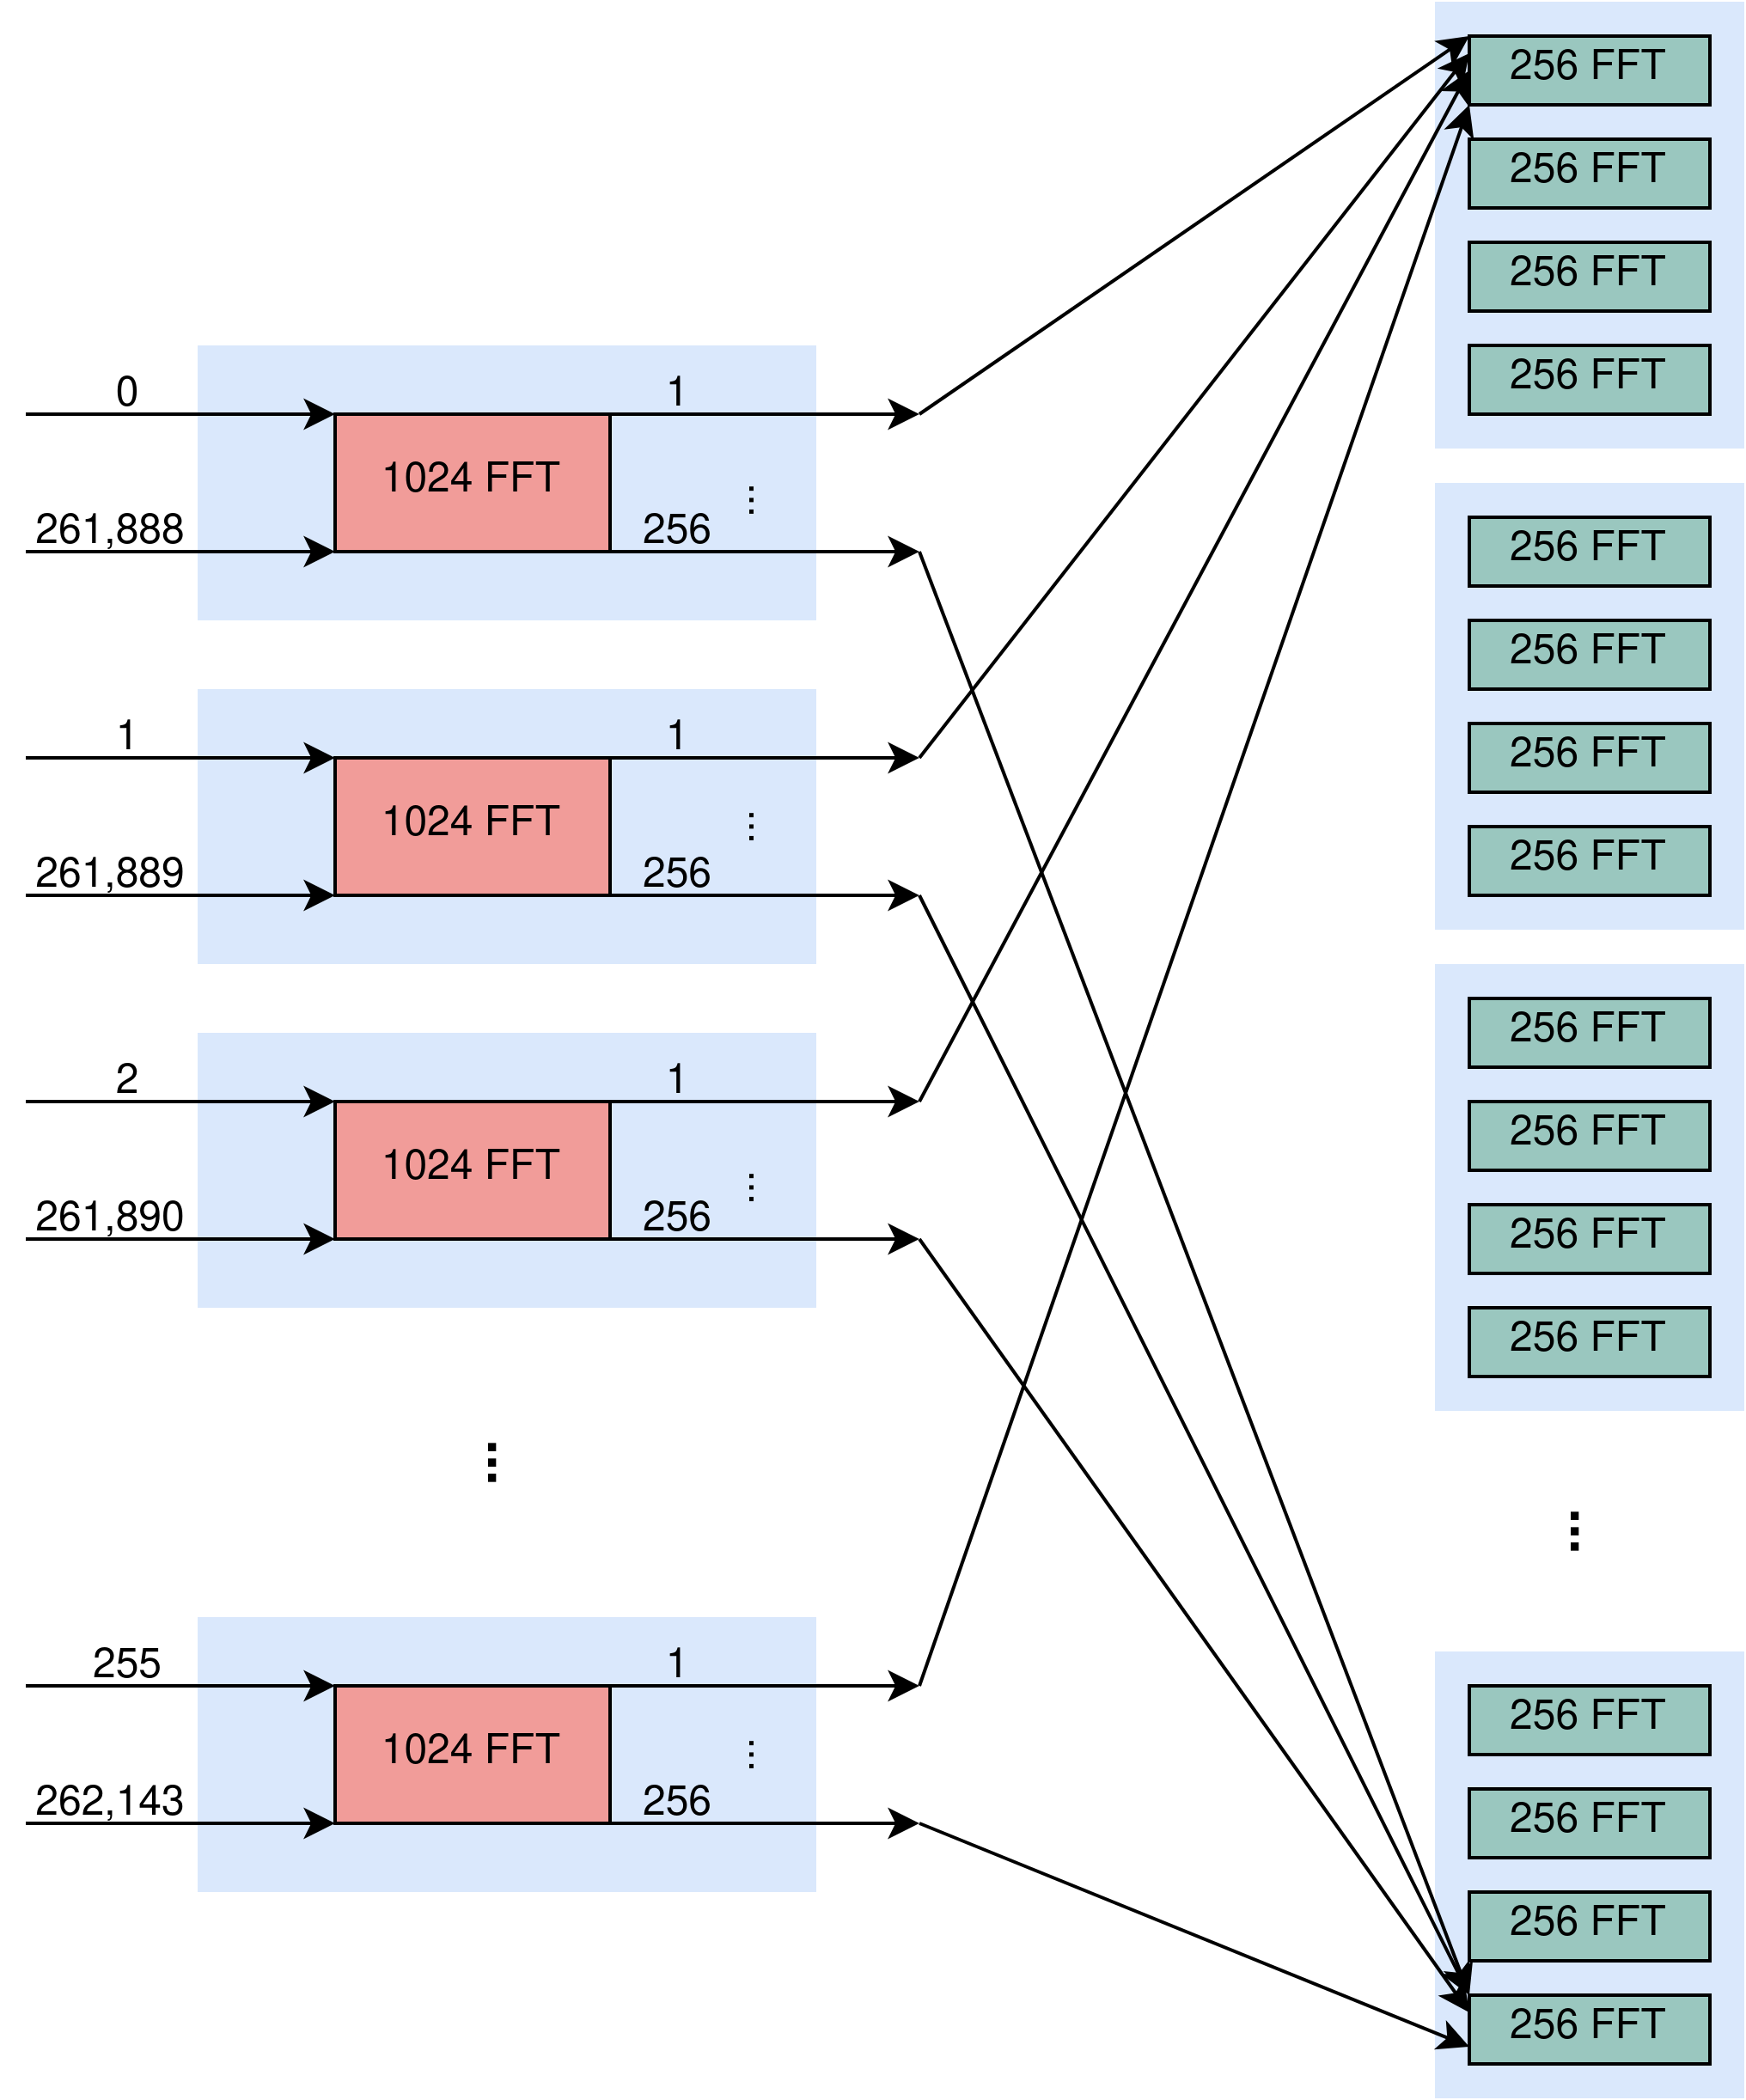
\includegraphics[width=0.7\textwidth]{images/stage_reorder.png}
    \captionsetup{justification=centering}
    \caption{Reorder scheme between stages}
            Every light blue box represents one AI Engine tile. It shows how the memory of one tile of the second stage is composed of multiple single memory entries from the first stage.
    \label{fig:stage_reorder}
\end{figure}

\subsection{Partitioner}
The Partitioner serves as a wrapper for interacting with the DDR memory, effectively encapsulating memory access from the rest of the design. This encapsulation enables the algorithm to be adapted for real-world scenarios without necessitating modifications to integral components. The primary functions of the Partitioner include loading data from DDR memory and reordering it for optimal use in the AI engines. The reordering schema utilized by the Partitioner is illustrated in figure \ref{fig:input_reorder}. Initially, the data is segmented into frames of 1024-point values for the first stages of the \ac{fft}. Each value is extracted in 256-step increments from the original memory to satisfy the input order constraints of the \ac{fft} algorithm. Once reordered, the data frame is divided into eight streams, with each stream containing 32 \ac{fft} packets. Specifically, the first stream carries packets 0 to 31, the second stream carries packets 32 to 63, and this pattern continues for the remaining streams up to packet 255. Importantly, during this splitting process, no additional information about the \ac{fft} is incorporated. This task is managed by the subsequent building block, the Packet Sender, to which the eight output streams are connected.

\begin{figure}[h]
    \centering
    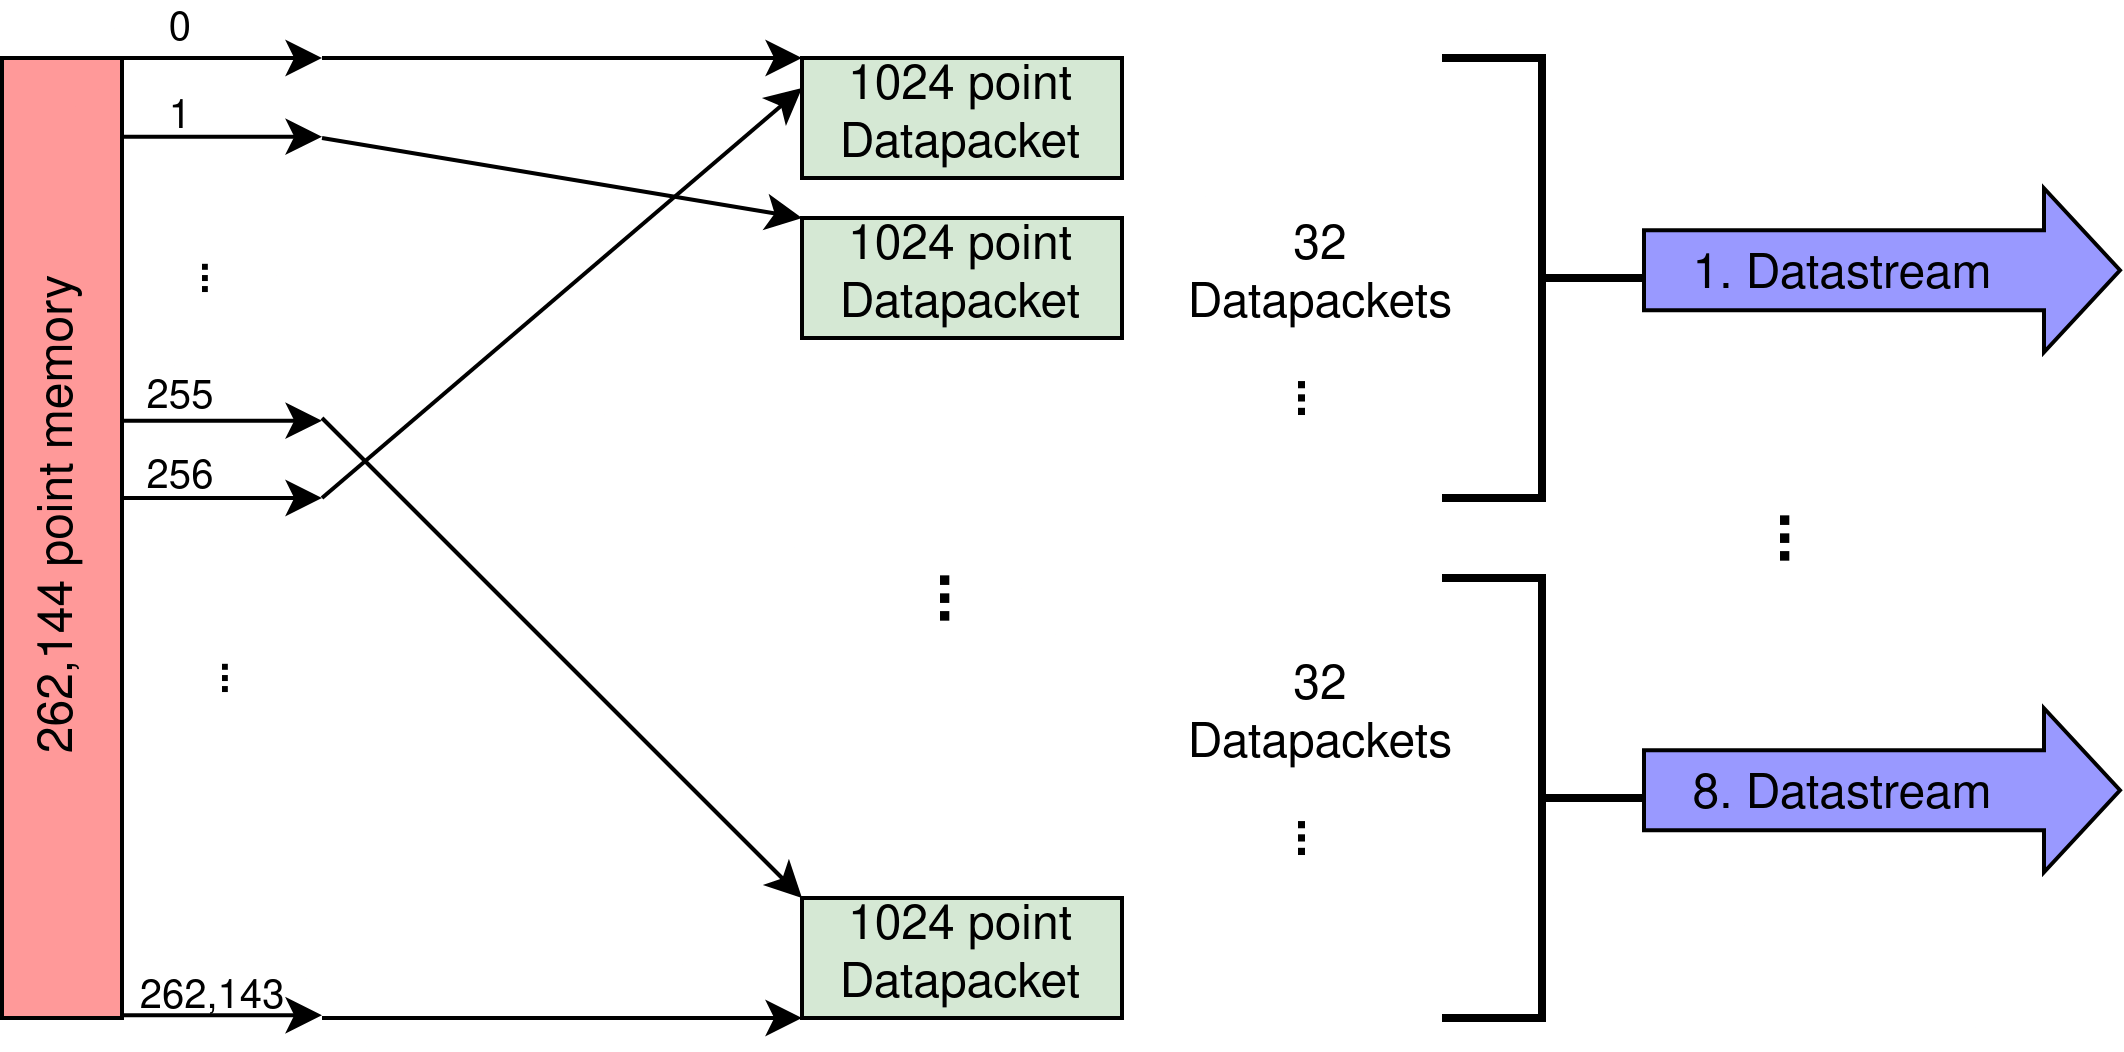
\includegraphics[width=0.7\textwidth]{images/input_reorder.png}
    \captionsetup{justification=centering}
    \caption{Reordering in the Partitioner}
            It is shown how the datastreams that are send from the Partitioner are created within. 32 datapackets are composed into one datastream.
    \label{fig:input_reorder}
\end{figure}

\subsection{Packetsender}
As its name implies, the Packetsender is responsible for constructing real data packets and transmitting them to the AI engines. This mechanism consists of two primary components: first, the streaming of data to the AI engine connection tiles via the AXI interface, and second, the streaming of data from those connection tiles to the tiles housing the AI engine cores. Since the second component is closely tied to the data packaging occurring outside the AI engines, it will also be discussed in this section.\par
In the first part of the process, a streaming connection is established between the connection tiles and the Packet Sender. The primary data for these streams can originate from either the Partitioner or the Rotator, allowing the Packet Sender to multiplex between the two sources. As explained in section \ref{sec:versal}, a single stream can be split into a maximum of 32 individual streams. To accommodate the data requirements for all 256 kernels, eight streams are used, each carrying data for 32 individual streams. Each of these individual streams contains 1,024 data points for a single \ac{fft}. To meet these requirements, the Packet Sender reads 1,024 values from a stream—either from the Partitioner or Rotator input—and appends a header that specifies the destination tile. The destination information is generated during the compile time of the AI engine kernels and is subsequently passed to the other building blocks as a table. Additionally, a control word is included with the transmitted data, providing information on which \ac{fft} stage the algorithm is currently executing, thereby enabling the correct branching within the AI engines. To conclude each packet, a stop byte is appended at the end of the data frame.

\subsection{Rotator}
The Rotator operates as an intermediary layer between the first and second stages of the \ac{fft}. Its primary function is to reorder the outputs from the first stage or prepare the data for memory write-back. The Rotator processes data received from eight streams, each connected to the connection tiles of the AI Engines. If the data originates from the first stage of the \ac{fft}, it is reordered and buffered in BRAM according to the memory scheme shown in Fig. X. Conversely, if the data is from the second stage, a reverse index reordering scheme is applied to ensure the correct output order. In the first scenario, the data is transmitted through eight streams to the Packet Sender, which then streams the data back into the AI Engines. The data splitting scheme follows a pattern similar to that used by the Partitioner, with the key difference being that a single 1024-point dataframe now holds four 256-point dataframes. When data originates from the second stage of the \ac{fft}, it is sent via a single stream to the Connector. The Connector executes a straightforward memory write-back operation for all received elements. This process encapsulates memory access, isolating it from the rest of the logical design, similar to the approach employed by the Partitioner.

\begin{figure}[h!]
    \centering
    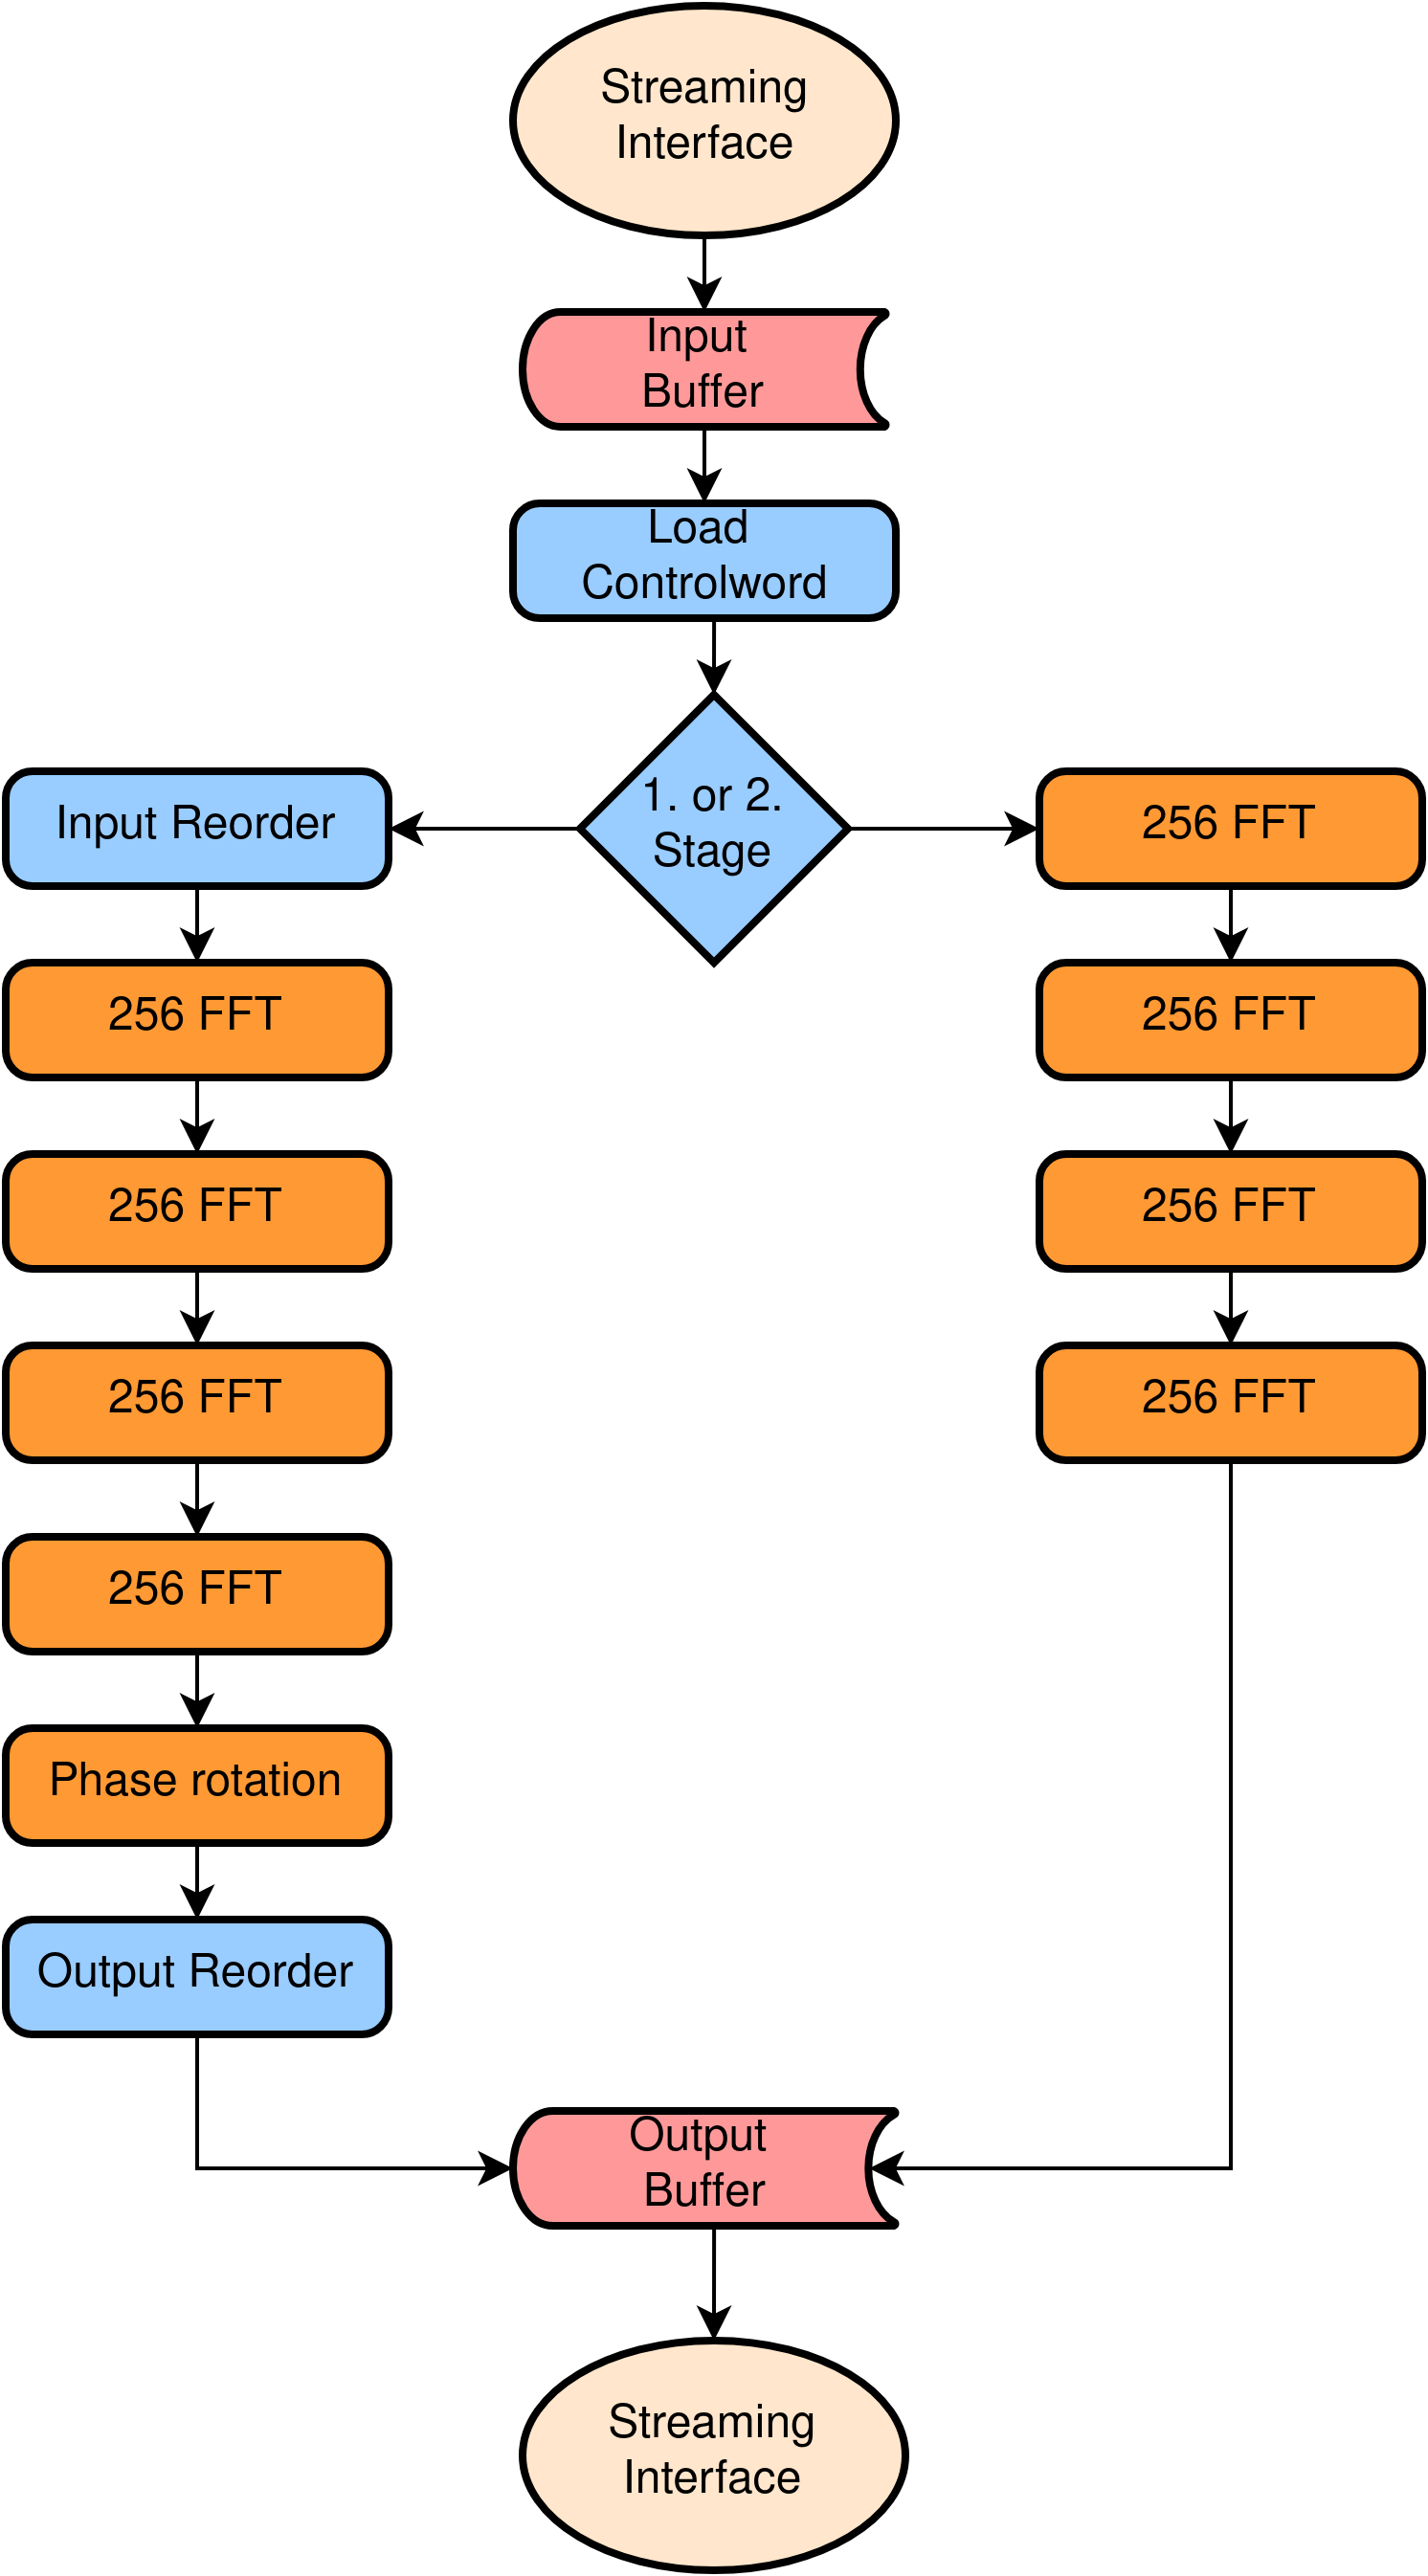
\includegraphics[width=0.45\textwidth]{images/flex_kernel.png}
    \captionsetup{justification=centering}
    \caption{Controlflow of the AI Engine kernel}
        The color in this seem indicate which part of the AI Engine is used for the operation. Red indicates loads and writes to the explicitly allocated memory. Orange are operations that run on the vector unit of the processor. Blue are controlflow functions that do not involve specific calculations. It is shown that both stage need four 256 FFTs. For stage 1 some reorder preparations needed to be done.
    \label{fig:flex_kernel}
\end{figure}

\section{AI Engine kernels}\label{sec:design_ai}
The AI engine kernel is the core component of this algorithm, responsible for the main computations, and is instantiated 256 times. As a result, the kernel must be rigorously optimized to ensure that its runtime remains below the instruction threshold of 73,125,000 instructions per kernel. To achieve this, the kernel heavily utilizes the vector unit of the small \ac{risc} processor. Additionally, the kernel must be adaptable for either a 1024-point \ac{fft} followed by a phase rotation or a set of four independent 256-point \ac{fft}s. Before going into the optimizations of the \ac{fft}s an important point to consider is the handling of the incoming data. The data can either be read element by element from a stream or can be directly copied into the AI Engines memory. For this the design the latter approach is chosen as it reduces the active managed instructions to one, which accepts the dataframe. So at the begin of the kernel the data for the \ac{fft} lies in an buffer. This is shown in figure \ref{fig:flex_kernel} as a red buffer, which is directly filled by the streaming interface.\par
An efficient approach is to split the 1024-point \ac{fft} using the Cooley-Tukey algorithm into four 256-point \ac{fft}s, which are then connected to 256 four-point \ac{fft}s. This strategy enables reuse of the 256-point \ac{fft} in both stages of the algorithm. The distinctions between the two stages are illustrated in Fig. B. As shown, the primary operation of the kernel is the 256-point \ac{fft}, which is invoked multiple times in both variants. Consequently, the next section will examine the design of this component in detail, as its optimization will impact other parts of the kernel as well.\par

\begin{figure}[h]
    \centering
    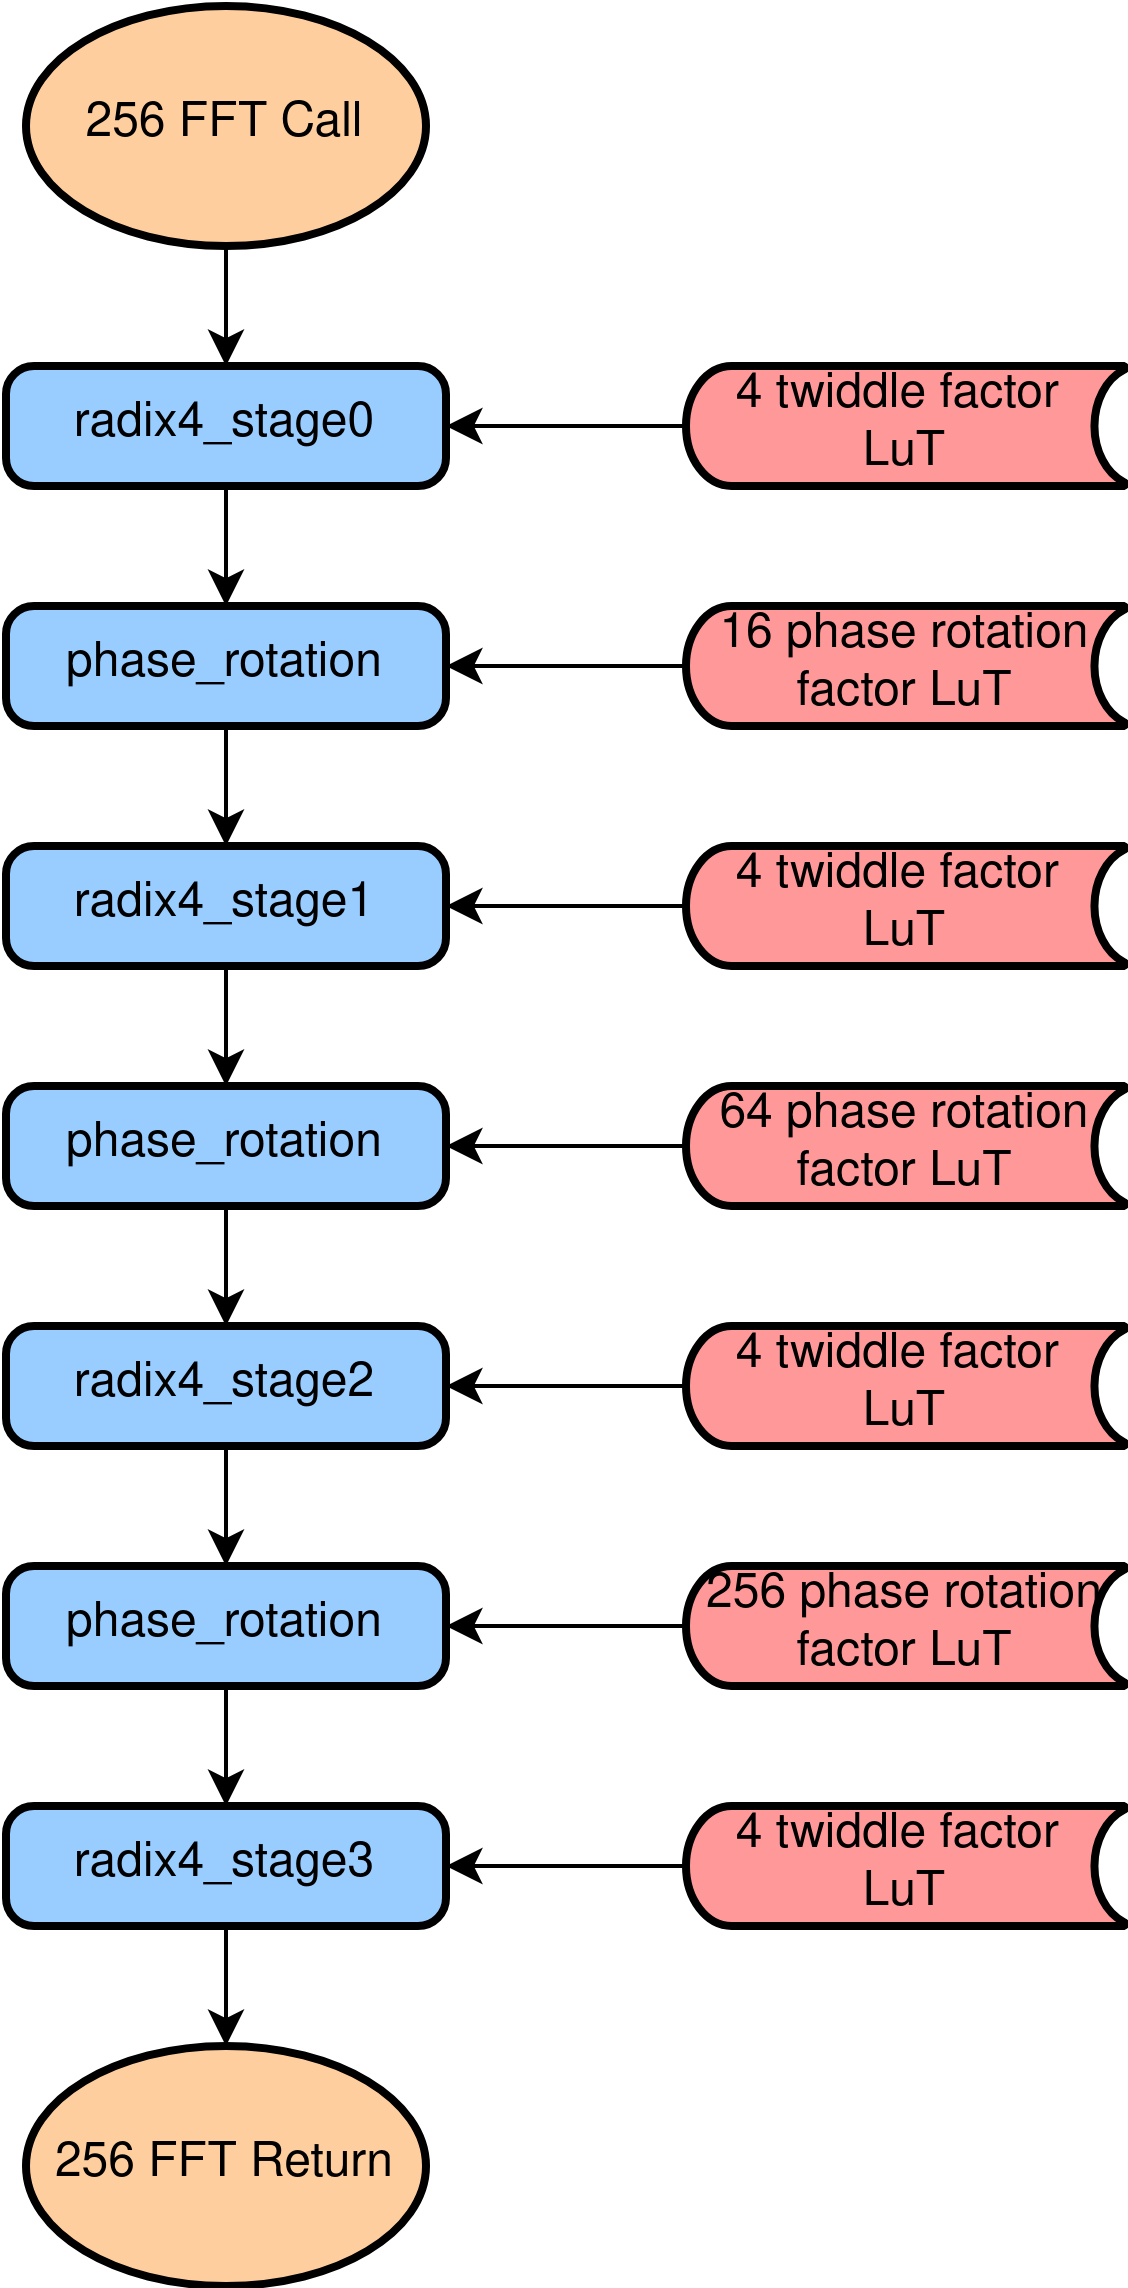
\includegraphics[width=0.35\textwidth]{images/256_func.png}
    \captionsetup{justification=centering}
    \caption{Controlflow of the 256 point \ac{fft}}
            Shows the internal structure of the 256 point FFT with access to special units denoted by color. Red highlights memory operation while orange indicates operations on the vector unit.
    \label{fig:256_kernel}
\end{figure}

The initial step in optimization is the application of the Cooley-Tukey algorithm, which not only facilitates parallelization but also reduces computational complexity, as discussed in section \ref{sec:ft}. This raises the question of the optimal decomposition approach. The decomposition should align with the capabilities of the AI Engine's vector unit. As outlined in section \ref{sec:versal}, the vector unit can perform MAC operations on two vectors of four elements in two instruction cycles. By utilizing twiddle factors in one vector and input values in the other, the smallest feasible \ac{fft} size would be four elements. Therefore, a radix-4 decomposition is the most efficient approach, where the entire 256-point \ac{fft} is constructed from 4-point \ac{fft}s. This process splits the 256-point \ac{fft} into four stages, as illustrated in Fig. C. To achieve this structure, the 256-point \ac{fft} is first divided into four 64-point transformations, each connected to 4-point \ac{fft}s. Each 64-point \ac{fft} is further decomposed into four 16-point \ac{fft}s, which are then split into four 4-point units. The 4-point unit is the smallest computational block, processing two vectors: one containing the input values and the other one containing the twiddle factors, which remain constant for all radix-4 calculations. Between stages, phase rotations are applied to the outputs of the preceding stage with a vectored multiply operation which can also take up to 4 values. To optimize runtime, I have used precalculated twiddle factors and phase rotations. Calculating the twiddle factors during runtime was considered but was overthrown as it would take to much out of the available runtime budget. This results in a total of 596 precalculated values, distributed across 4 twiddle factors, 16 phase rotation factors for the first stage, 64 for the second stage, 256 for the third stage, and 256 for the final stage. Memory savings are achieved in the last stage by exploiting periodicities in the precalculated values.\par
As previously discussed, when calculating four 256-point \ac{fft}s, the routine is invoked four times with different input values, and the results are subsequently streamed to the output. However, additional steps are required when performing a 1024-point \ac{fft} followed by a phase shift. Initially, the data must be reordered. After completing the smaller transforms, the results are multiplied by the phase rotation factors within the 1024-point \ac{fft}, and the 256 four-point \ac{fft}s are applied to the outputs. Finally, the results are multiplied by the precalculated phase rotation factor for the encompassing $2^{18}$-point \ac{fft}. For the initial reordering, the incoming data is partitioned into four blocks, with every fourth element from the unordered data assigned to the same block. After performing the smaller \ac{fft}s on the reordered data, the phase rotation is applied using the precalculated values, similar to the phase rotation between stages of the 256-point \ac{fft}. Following this multiplication, a four-point unit processes the results to connect them. The outputs are then index-reversed, reordered, and multiplied by the 1024-point phase rotation. Like the other phase rotation factors, the values for the 1024-point rotation are also precalculated. Since these factors do not exhibit periodicities, the entire 1024-value table must be stored. Additionally, this table is unique for each instantiation of the AI engine kernel, in contrast to the other lookup tables.